% !TEX TS-program = pdflatex
% !TEX encoding = UTF-8 Unicode

% This is a simple template for a LaTeX document using the "article" class.
% See "book", "report", "letter" for other types of document.

\documentclass[11pt, titlepage]{article} % use larger type; default would be 10pt

\usepackage[utf8]{inputenc} % set input encoding (not needed with XeLaTeX)

%%% Examples of Article customizations
% These packages are optional, depending whether you want the features they provide.
% See the LaTeX Companion or other references for full information.

%%% PAGE DIMENSIONS
\usepackage{geometry} % to change the page dimensions
\geometry{a4paper} % or letterpaper (US) or a5paper or....
\geometry{margin=2cm, headsep=5mm, includefoot, includehead}

\usepackage{graphicx} % support the \includegraphics command and options

% \usepackage[parfill]{parskip} % Activate to begin paragraphs with an empty line rather than an indent

%%% PACKAGES
\usepackage{booktabs} % for much better looking tables
\usepackage{array} % for better arrays (eg matrices) in maths
\usepackage{paralist} % very flexible & customisable lists (eg. enumerate/itemize, etc.)
\usepackage{verbatim} % adds environment for commenting out blocks of text & for better verbatim
\usepackage{subfig} % make it possible to include more than one captioned figure/table in a single float
% These packages are all incorporated in the memoir class to one degree or another...

%%% HEADERS & FOOTERS
\usepackage{fancyhdr} % This should be set AFTER setting up the page geometry
\pagestyle{fancy} % options: empty , plain , fancy
\fancyhead{}
%%% SECTION TITLE APPEARANCE
\usepackage{sectsty}
\allsectionsfont{\sffamily\mdseries\upshape} % (See the fntguide.pdf for font help)
% (This matches ConTeXt defaults)

%%% ToC (table of contents) APPEARANCE
\usepackage[nottoc,notlof,notlot]{tocbibind} % Put the bibliography in the ToC
\usepackage[titles,subfigure]{tocloft} % Alter the style of the Table of Contents
\renewcommand{\cftsecfont}{\rmfamily\mdseries\upshape}
\renewcommand{\cftsecpagefont}{\rmfamily\mdseries\upshape} % No bold!

\usepackage{lastpage}
\usepackage{rotating}
%---------- Enable IEEEtran.bst configurations ------
\usepackage{IEEEtrantools}
%----------------------------------------------------

%%% END Article customizations

%%% The "real" document content comes below...

%%% Header %%%%%%%%%%%%%%%%%%%%%%%%%%%%%
\setlength{\headheight}{52.4842pt}
\lhead{EH2760 Management of Projects \\
       Assignment 1 \\
       ESS-CAR/ESS-NW \\
       Leon Fernandez, leonfe@kth.se}
\rhead{Status Report 4 \\
       \today \\
       Version 1 \\
       \thepage(\pageref{LastPage})}
\renewcommand{\headrulewidth}{0.4pt}
%%%%%%%%%%%%%%%%%%%%%%%%%%%%%%%%%%%%%%%%

%%% Footer %%%%%%%%%%%%%%%%%%%%%%%%%%%%%
%\cfoot{blablablabla}
%\renewcommand{\footrulewidth}{0.4pt}
%%%%%%%%%%%%%%%%%%%%%%%%%%%%%%%%%%%%%%%%

%\title{ESS-CAR/ESS-NW Project Plan}
%\author{Jonas Ekman \\
%        Leon Fernandez \\
%        Yini Gao \\
%        Fredrik Hyyrynen \\
%        Jacob Kimblad \\
%        Yifan Ruan
%        }
%\date{} % Activate to display a given date or no date (if empty),
         % otherwise the current date is printed 

\begin{document}
%\maketitle
\bstctlcite{BSTcontrol} % IEEEtran.bst controls enabled


%----------------------------------------------------------------------------------------
%	TITLE PAGE
%----------------------------------------------------------------------------------------
\iffalse
\begin{titlepage} % Suppresses displaying the page number on the title page and the subsequent page counts as page 1
	\newcommand{\HRule}{\rule{\linewidth}{0.5mm}} % Defines a new command for horizontal lines, change thickness here
	
	\center % Centre everything on the page
	
	%------------------------------------------------
	%	Headings
	%------------------------------------------------
	
	\textsc{\LARGE EH2760 Management of Projects}\\[1.5cm] % Main heading such as the name of your university/college
	
	\textsc{\Large ESS-CAR/ESS-NW}\\[0.5cm] % Major heading such as course name
	
	\textsc{\large Stockholm, Sweden}\\[0.5cm] % Minor heading such as course title
	
	%------------------------------------------------
	%	Title
	%------------------------------------------------
	
	\HRule\\[0.4cm]
	
	{\huge\bfseries Status Report 4}\\[0.4cm] % Title of your document
	
	\HRule\\[1.5cm]
	
	%------------------------------------------------
	%	Author(s)
	%------------------------------------------------
	
	\begin{minipage}{0.4\textwidth}
		\begin{flushleft}
			\large
                        \textsc{Jonas Ekman}
			\\
			\textsc{Yini Gao}
                        \\
                        \textsc{Jacob Kimblad}
		\end{flushleft}
	\end{minipage}
	~
	\begin{minipage}{0.4\textwidth}
		\begin{flushright}
			\large
                        \textsc{Leon Fernandez}
			\\
			\textsc{Fredrik Hyyrynen}
                        \\
                        \textsc{Yifan Ruan}
		\end{flushright}
	\end{minipage}
	
	% If you don't want a supervisor, uncomment the two lines below
        % and comment the code above
	%{\large\textit{Author}}\\
	%John \textsc{Smith} % Your name
	
	%------------------------------------------------
	%	Date
	%------------------------------------------------
	
	\vfill\vfill\vfill % Position the date 3/4 down the remaining page
	
	{\large\today} % Date, change the \today to a set date if you want
                       % to be precise
	
	%------------------------------------------------
	%	Logo
	%------------------------------------------------
	
	%\vfill\vfill
	%
\includegraphics[width=0.2\textwidth]{placeholder.jpg}\\[1cm]
        % Include a department/university logo
        % - this will require the graphicx package
	 
	%-------------------------------------------------------------------
	
	\vfill % Push the date up 1/4 of the remaining page
	
\end{titlepage}
\fi
%-------------------------------------------------------------------------


\section*{General Description of Status}
The overall status of the project is stable. Since the last status report there has been some turbulence, however. Due to some
issues with getting some of the on-board communication working between processes, the project stalled for a couple of days.
At the time of writing, these issues have been resolved and the project is now proceeding rather smoothly.

\section*{Resource Status}
Due to some extract work needed to resolve the communication problems on-board, the project has exceeded the estimated time budget.

\section*{Problems / Action Plan}
Some features have been dropped in order to keep the exceeding of the time budget to a minimum. The most notable feature
is that network monitoring is now done via a web page instead of a smartphone app.

\section*{Risks / Action Plan}
All risks are currently being handled according to the plan. Documentation of the code using Doxygen is now in effect and has been for more than a week.

\section*{Project Changes From the Project Plan}
There has been some changes to the milestones. In \ref{fig:timeplan} it can be seen that some of the milestones has had their relative order changed. This was because the
new order made more sense from a technical perspective. Furthermore, many of the milestones have been given a later date since the project had some issues with stalling that are now resolved.

\appendix
\section{EVM}
\begin{figure}[h]
     \centering
     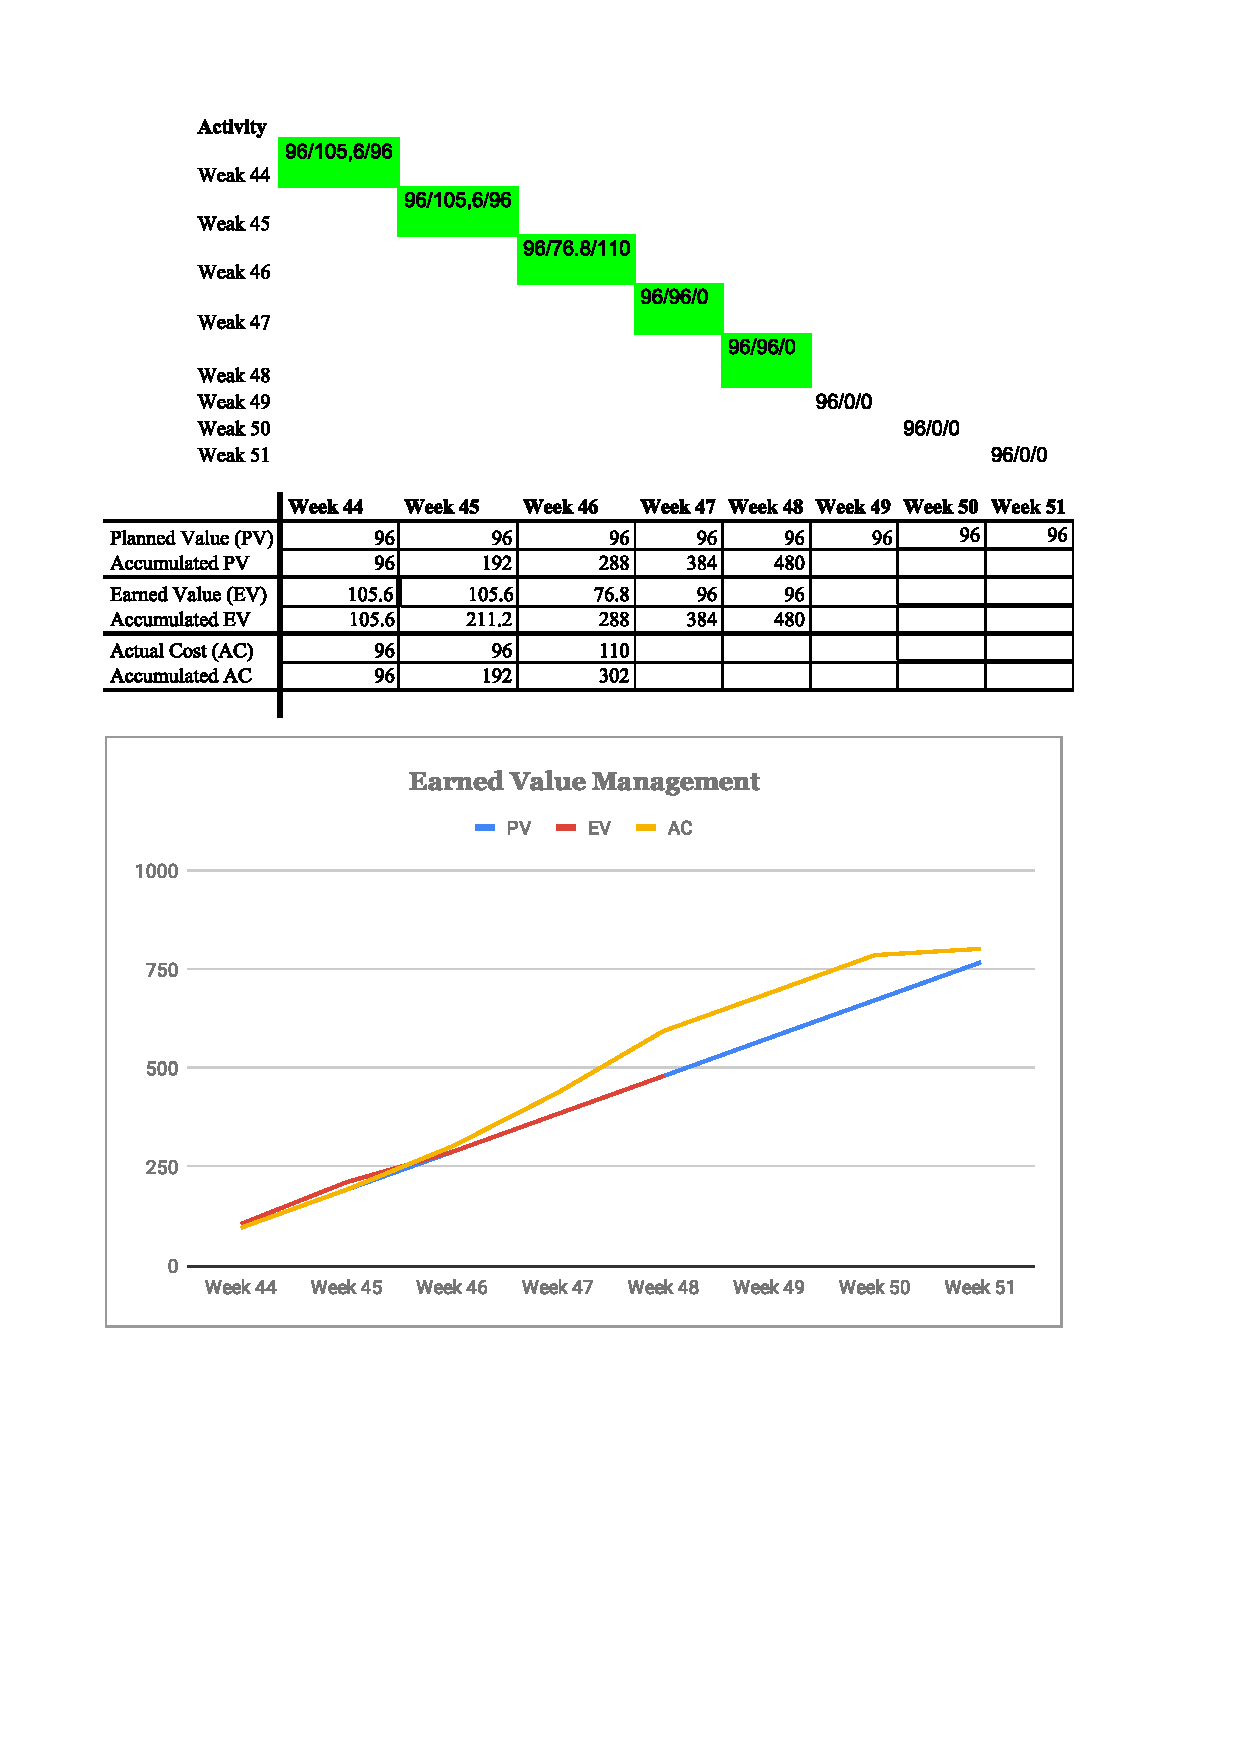
\includegraphics[scale=0.8]{evm.pdf}
     \caption{Earned Value Management analysis.}
     \label{fig:evm}
\end{figure}

\section{Time Plan}
\begin{sidewaysfigure}
     \centering
     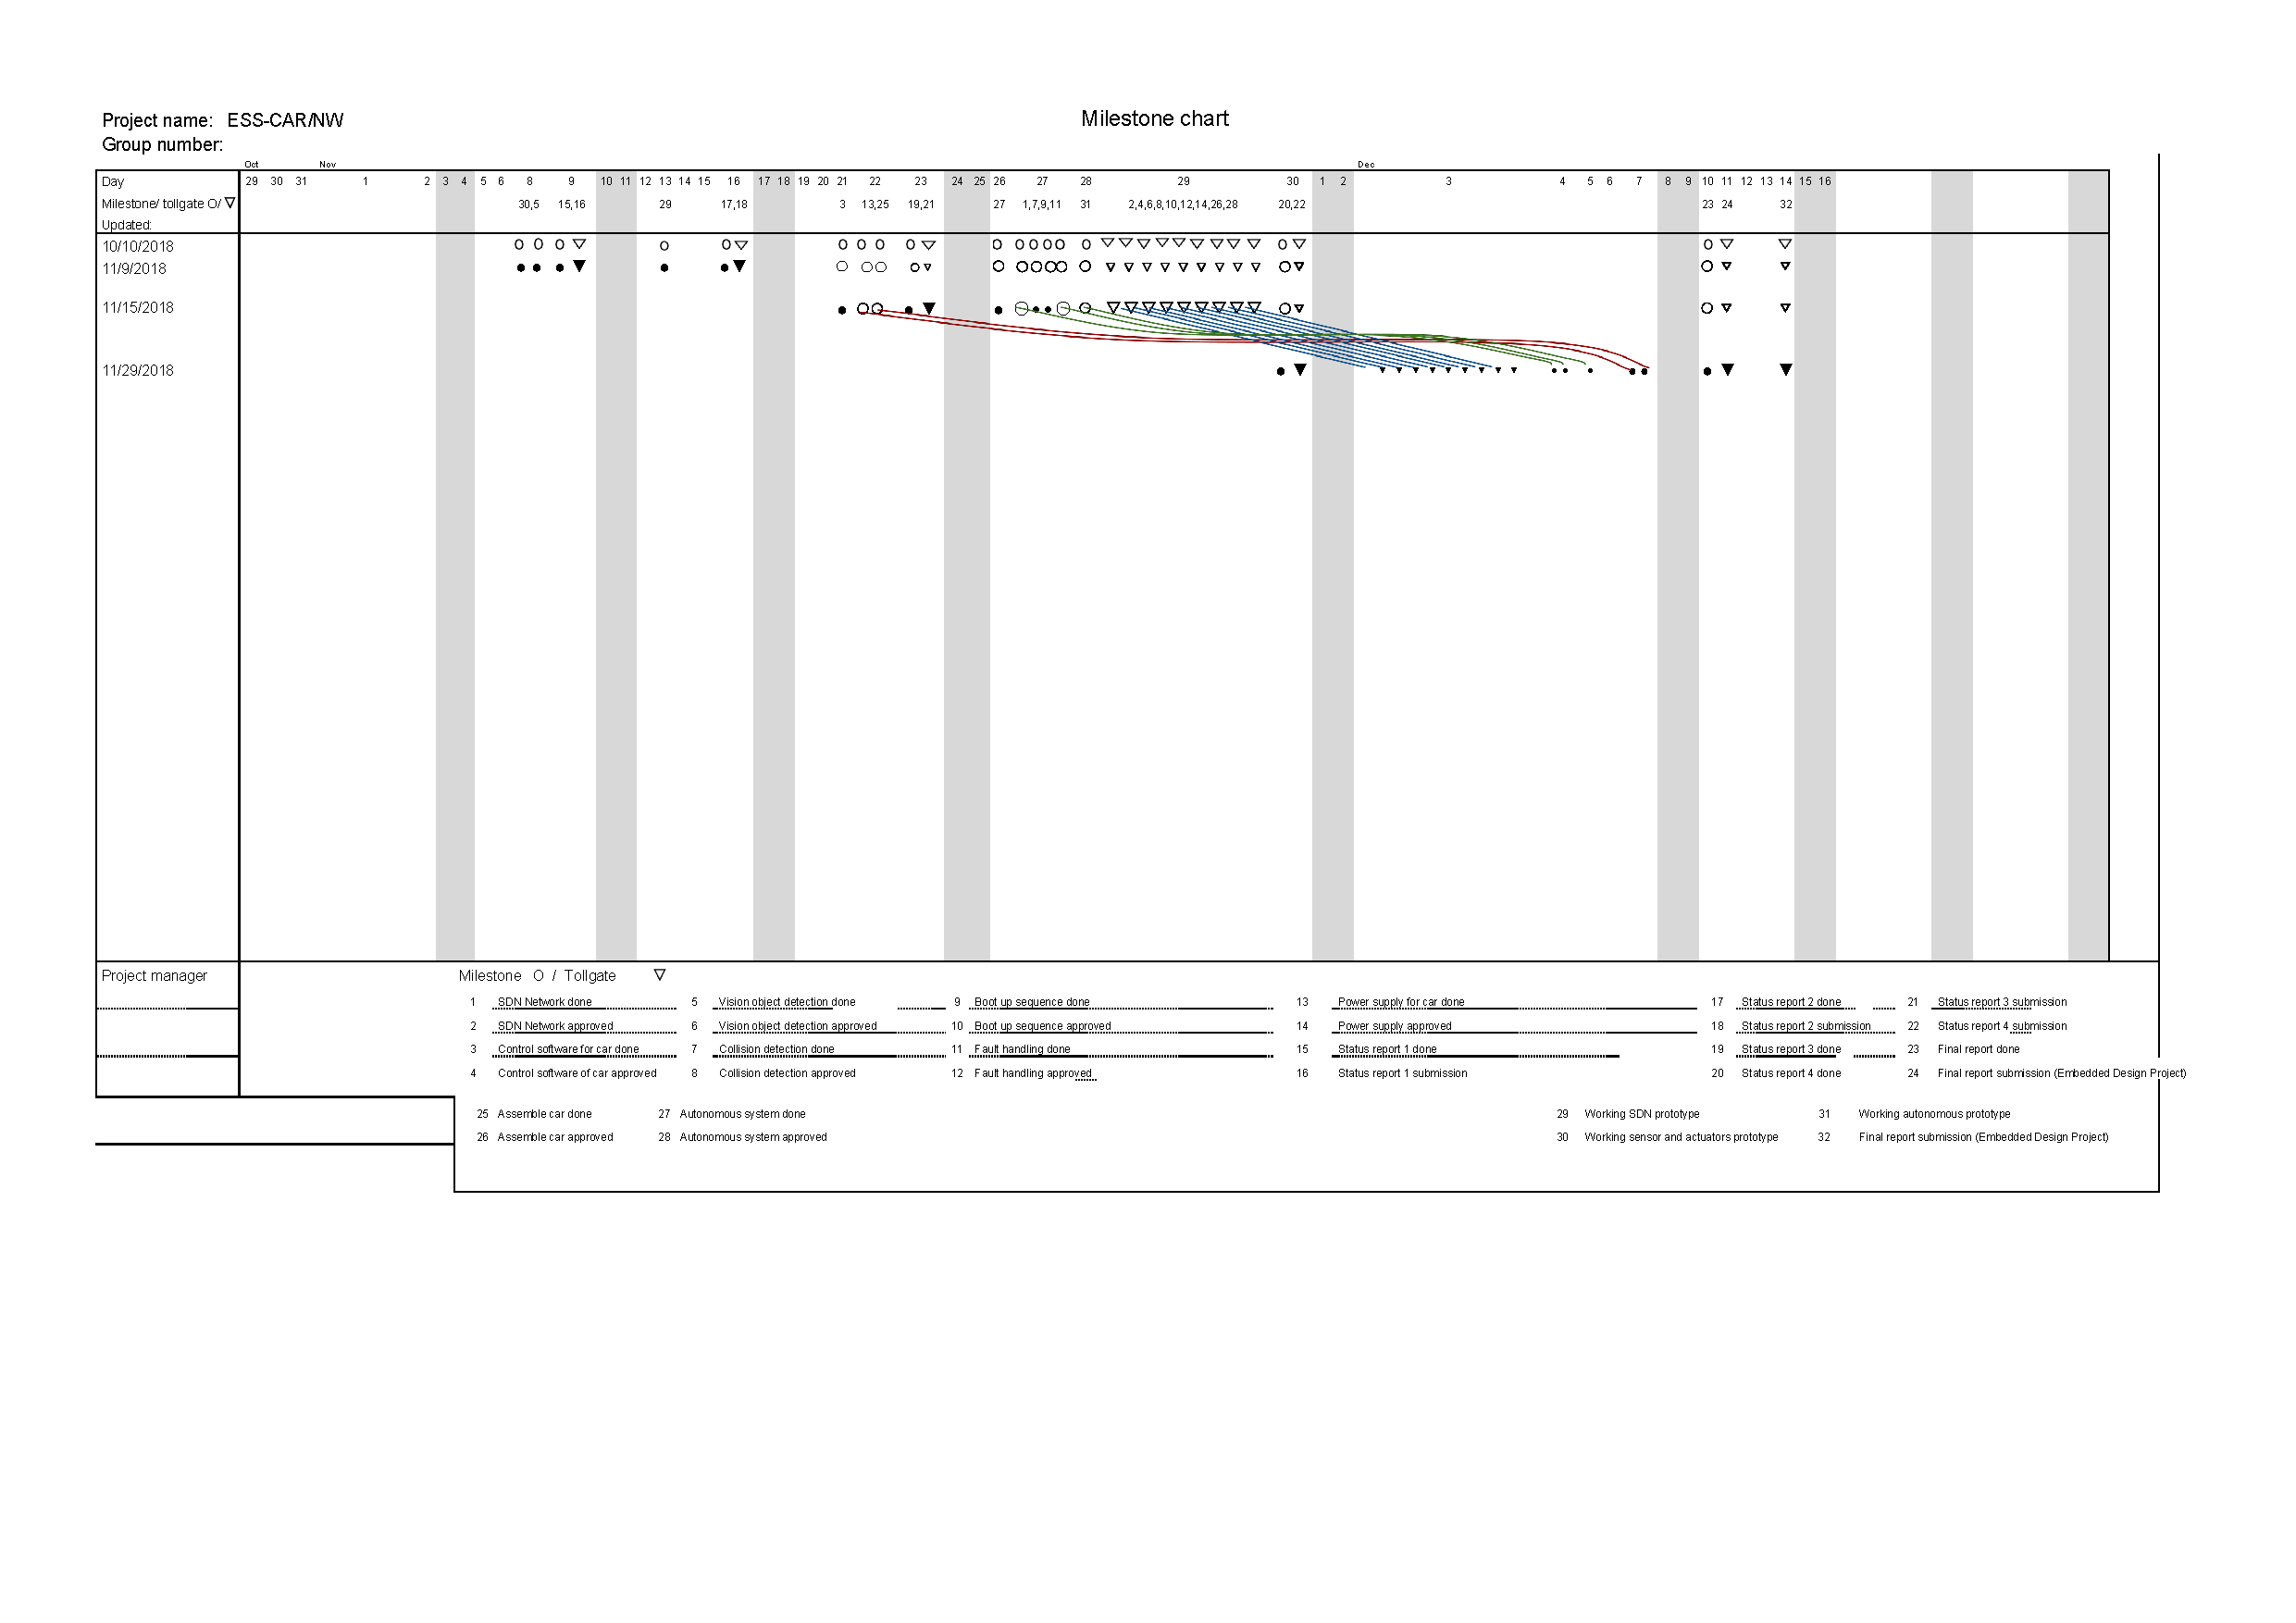
\includegraphics[scale=0.6]{timeplan.pdf}
     \caption{Timeplan for the project.}
     \label{fig:timeplan}
\end{sidewaysfigure}

\section{Resource Plan}
\begin{sidewaysfigure}
     \centering
     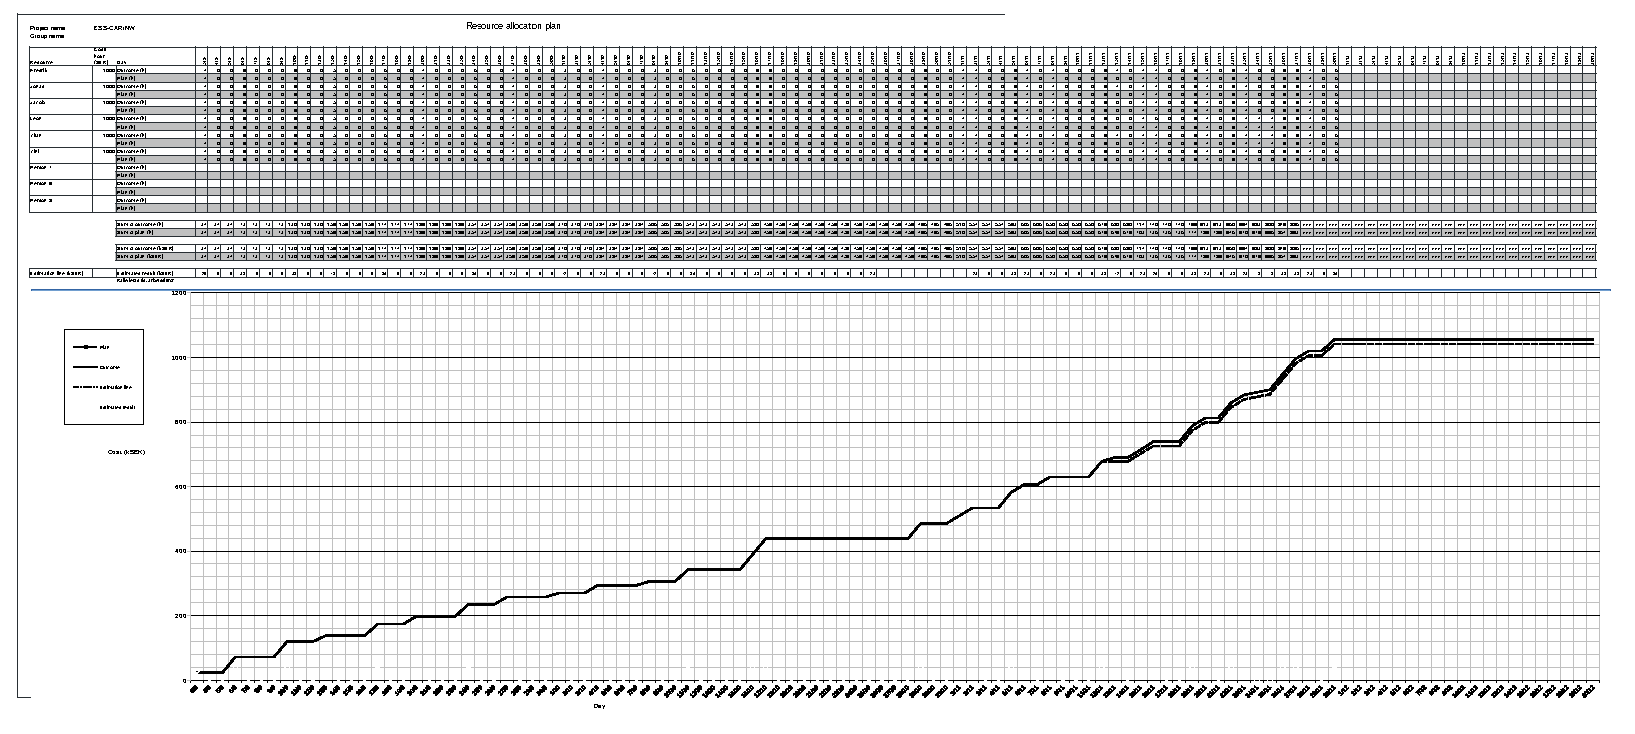
\includegraphics[scale=0.8]{resource_plan.pdf}
     \caption{Resource plan for the project.}
     \label{fig:resource}
 \end{sidewaysfigure}
\end{document}
